\chapter{Introduction}
\label{ch:intro}


\section{Demo}

\subsection{2 column}

\begin{multicols}{2}
[
    All human things are subject to decay. And when fate summons, Monarchs must obey.
]

    \blindtext

    \blindtext
\end{multicols}

\subsection{Code listing}

\begin{lstlisting}[language=bash]
[mamos@binfservas31 mamos]$ apptainer exec /containers/apptainer/subread_2.0.6.sif featureCounts -v
\end{lstlisting}

\begin{lstlisting}
    featureCounts v2.0.6
\end{lstlisting}

\subsection{Table and footnote}

\begin{longtable}[c]{|l|l|l|l|}
    \hline
    Software & Version & Module or container & Container path\footnotemark{} \\
    \hline
    \endfirsthead

    \hline
    Software & Version & Module or container & Container path\footnotemark[\value{footnote}]{} \\
    \hline
    \endhead

    \multicolumn{4}{r}{\small \it The table continues on the next page} \\
    \normalsize
    \endfoot
    \hline
    \caption{Table of used software and versions}
    \endlastfoot

    FastQC & 0.11.9-Java-11 & Module &  -\\
    FastQC & 0.11.9-Java-11 & Module &  -\\
    fastp & 0.23.4-GCC-10.3.0 & Module &  -\\
    featureCounts & 2.0.6 & Container &  \lstinline!subread_2.0.6.sif! \\
    samtools & 1.20 & Container &  \lstinline!hisat2_samtools_408dfd02f175cd88.sif!\\
    hisat2 & 2.2.1 & Container &  \lstinline!hisat2_samtools_408dfd02f175cd88.sif!

    \footnotetext{On the cluster, all the path mentioned are located in /containers/apptainer/}
    \label{table:softwaresVersions}
\end{longtable}

\subsection{Figure}

\begin{figure}[h]
    \centering
    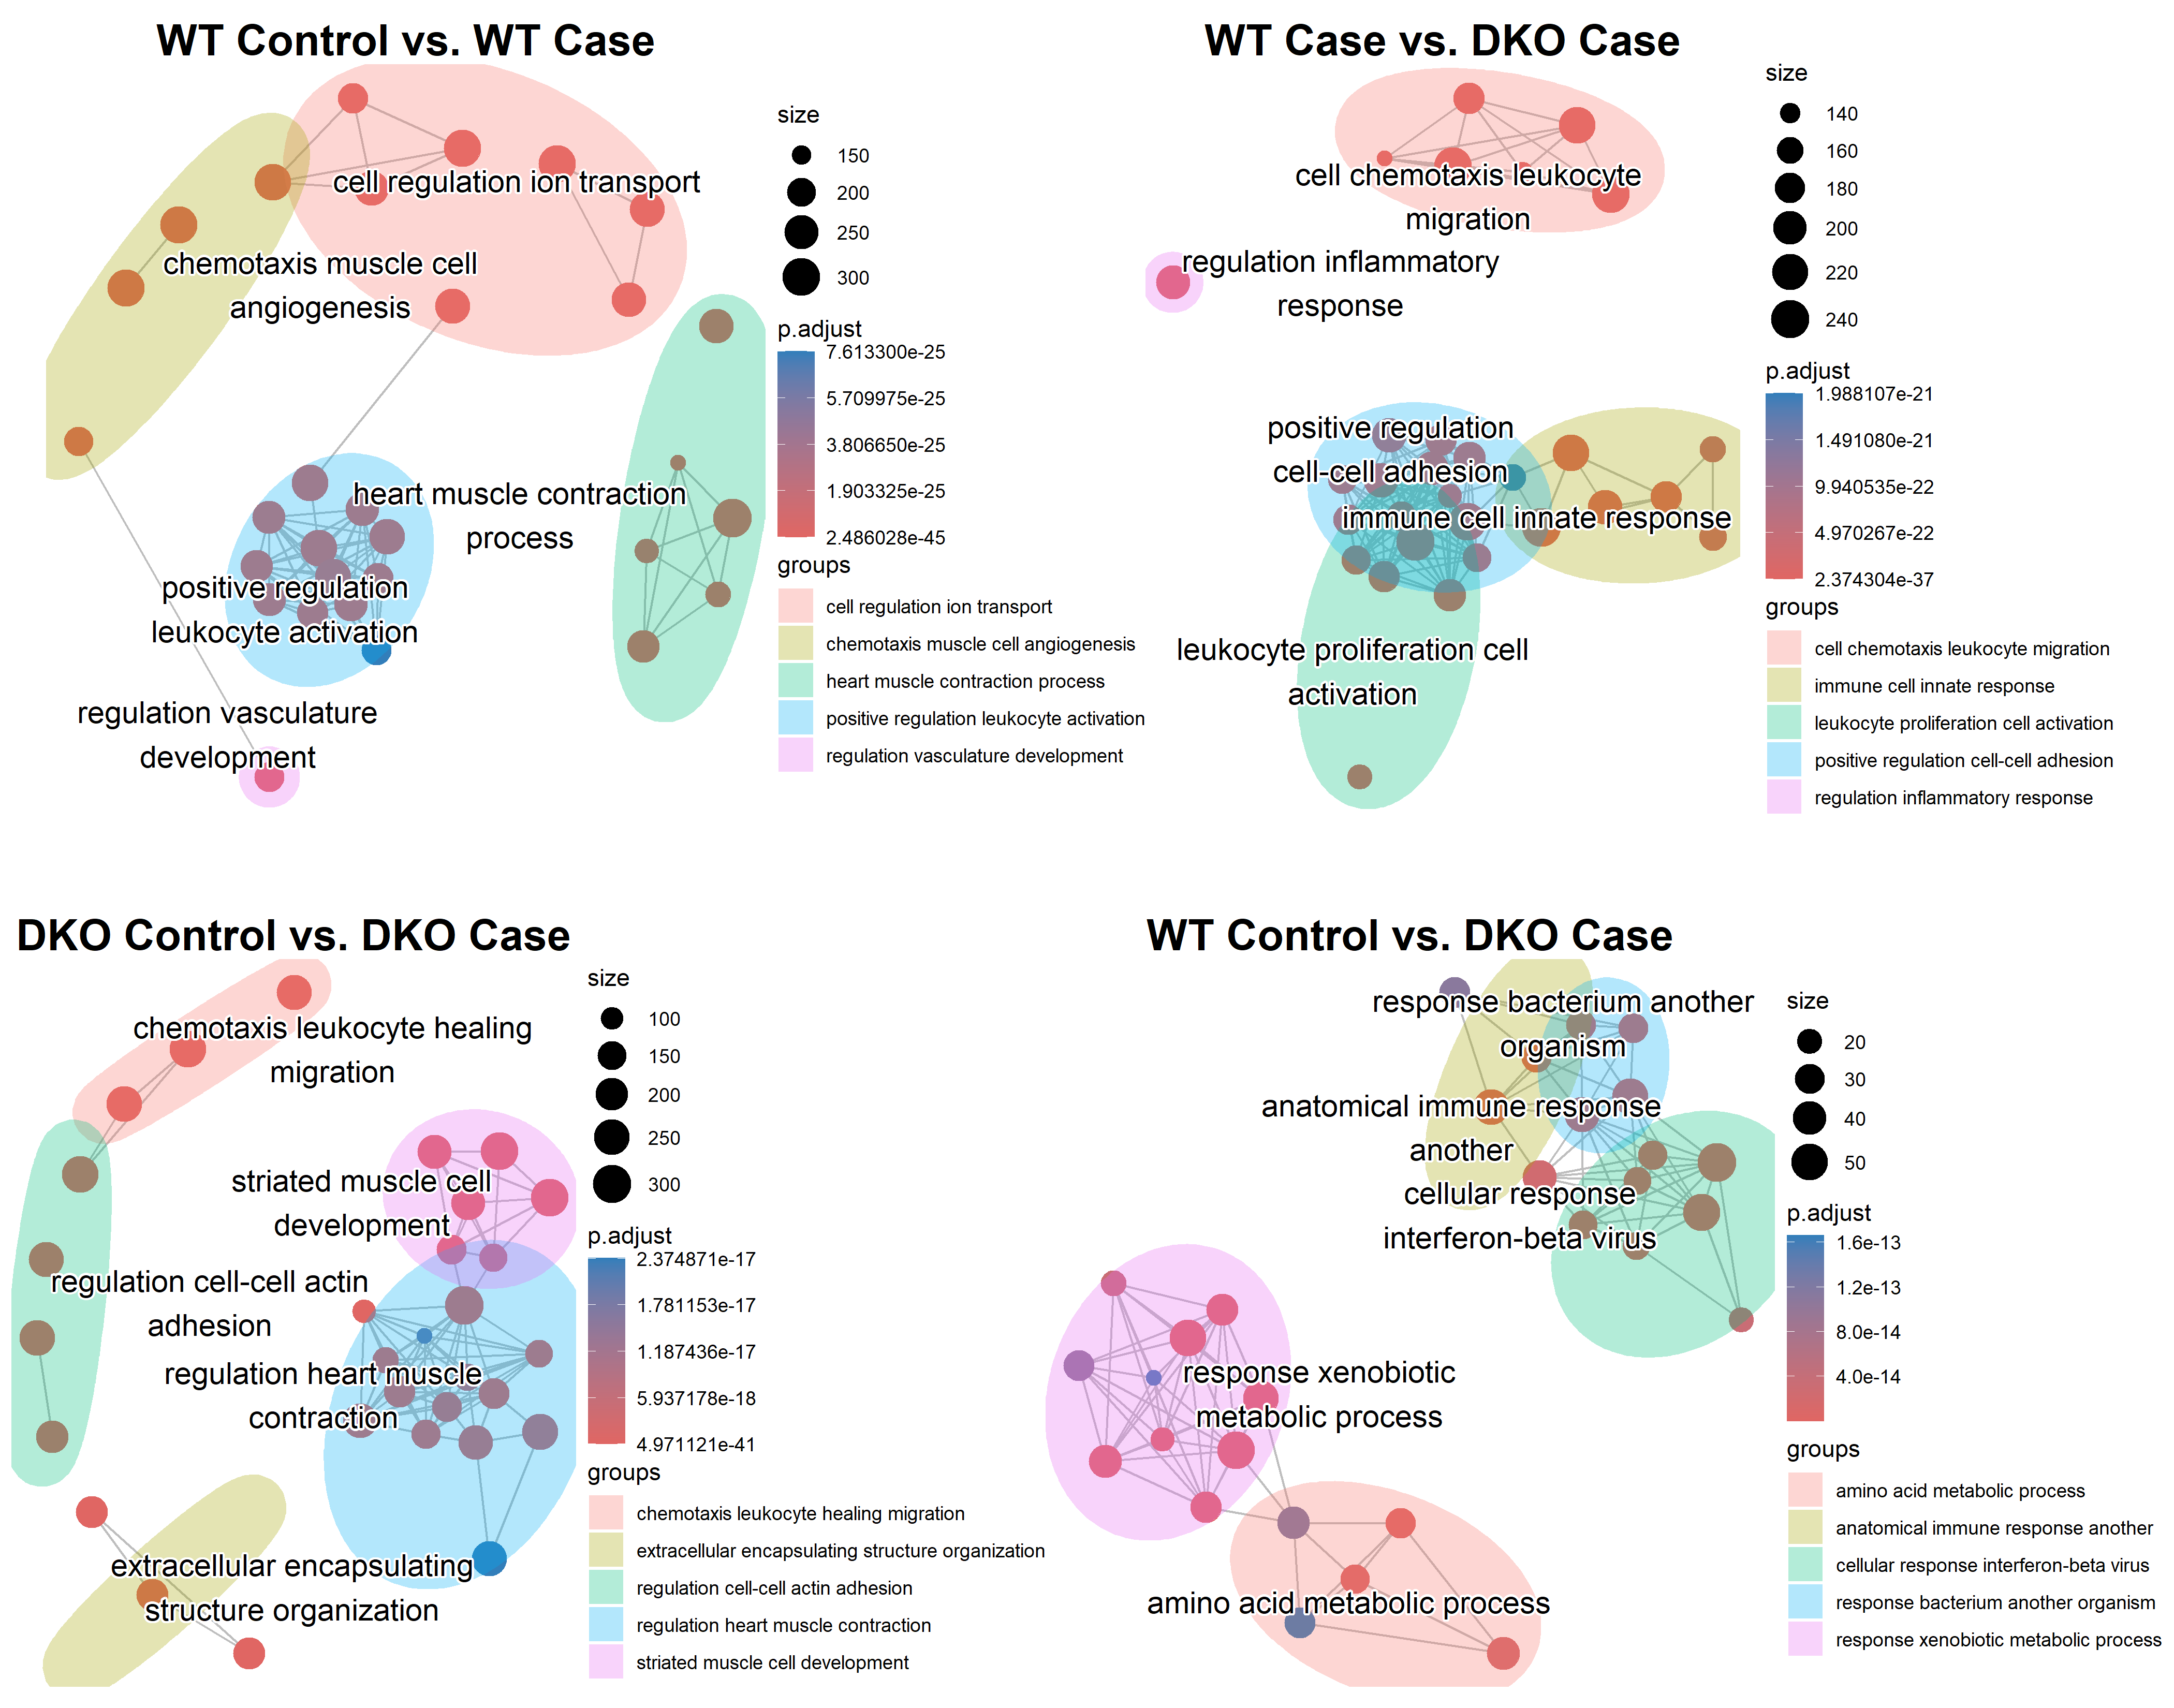
\includegraphics[width=1\linewidth]{figures/go_summary.png}
    \caption{Enrichement map from overrepresentation analysis}
    \label{fig:goSummary}
\end{figure}